\chapter{Implementation}
\label{chapter:implementation}
\thispagestyle{myheadings}

% set this to the location of the figures for this chapter. it may
% also want to be ../Figures/2_Body/ or something. make sure that
% it has a trailing directory separator (i.e., '/')!
\graphicspath{{./4_Implementation/}}
This chapter explores the setup required to conduct the experiments. The chapter is divided into 
\begin{itemize}
\item Data Generation:- We generate the data stream for the Linear road benchmark.
\item Query Execution:- We have implemented a query execution in C++ and extracted information while executing the query.
\item Deep Reinforcement Learning:- Written a Deep reinforcement learning agent to help optimize the order of operations.
\end{itemize}

\section{Data Generation}
The data is generated using the walmart linear road code generator without \\ mistim\cite{walmart_linearoad}.\\
Linear Road tests Stream Data Management Systems (SDMS) by measuring how many expressways a SDMS can support by giving accurate and timely results to four types of queries that fit two categories: continuous and historical.\cite{linearroad_website}
\begin{lstlisting}[language=bash, caption= generate linear road data, label={lst:linear road data generation}]
java com.walmart.linearroad.generator.LinearGen [-o <output file>] [-x <number of xways>] [-m <dummy value to activate multi-threading>]
\end{lstlisting}
Example output of this code
\begin{lstlisting}[caption= linear road data example output]
0,0,13,10,8,0,0,89,469920,-1,-1,-1,-1,-1,-1
0,0,17,10,8,0,1,65,348479,-1,-1,-1,-1,-1,-1
0,0,22,10,8,0,0,12,63360,-1,-1,-1,-1,-1,-1
0,0,33,10,8,0,1,94,501599,-1,-1,-1,-1,-1,-1
0,0,42,10,8,0,0,14,73920,-1,-1,-1,-1,-1,-1
0,0,4,10,7,0,0,61,322080,-1,-1,-1,-1,-1,-1
0,0,85,10,8,0,1,30,163679,-1,-1,-1,-1,-1,-1
0,0,11,10,6,0,1,41,221759,-1,-1,-1,-1,-1,-1
0,0,23,10,7,0,1,81,432959,-1,-1,-1,-1,-1,-1
0,0,15,10,6,0,0,5,26400,-1,-1,-1,-1,-1,-1
\end{lstlisting}
Each line in the example indicates $1$ data entry, the schema used in the generation of the above code as given.
\subsection{Schema}
The above generated data can be interpretated as follows:-\\
\begin{tabular}{ |c|c| } 
 \hline
  \multirow{5}{4em}{Column$1$} & Tells the type of query. \\  
            &	0: position report\\
			&	2: account balance request\\
			&	3: daily expenditure request\\
			&	4: travel time request	\\
 \hline
  Column$2$ & Timestamp position. \\  
 \hline
  Column$3$ & Vehicle identification number\\  
 \hline
  Column$4$ & Speed of the vehicle \\  
 \hline
  Column$5$ & Express way number \\  
 \hline
  Column$6$ & Lane ID $(0,...,4)$\\  
 \hline
  Column$7$ & Direction of movement($0=$East or $1=$West) \\  
 \hline
  Column$8$ & Segment ID $(0,...,99)$ \\
 \hline
  Column$9$ & Position of the vehicle. \\  
 \hline
  Column$10$ & Query identifier \\  
 \hline
  Column$11$ & Start Segment \\  
 \hline
  Column$12$ & End Segment \\  
 \hline
  Column$13$ & Day of the week \\  
 \hline
  Column$14$ & Minute of the day \\  
 \hline
  Column$15$ & Day in the past $10$ weeks \\  
 \hline
\end{tabular}

\section{Query Execution}
After the data is prepared, we need to execute the queries listed and explained in the previous chapter. We simplified and presented multiple plans of execution and we will explore them.\\
As suggested, a SDMS can take in multiple data stream as input but we were going to treat it as a single input. Below is the implementation of the $2$ queries in $C++$.
\subsection{Simpler Query}
The simpler query
\begin{lstlisting}[language=SQL,caption=simple query]
    SELECT exp_way, dir, seg, AVG(speed) as speed,
    FROM CarSegStr [RANGE 5 MINUTES]
    WHERE car_id = target
    GROUP BY exp_way, dir, seg;
\end{lstlisting}
The goal of implementing this query is to get a sense of time required for executing queries, the time for taking input and time for providing an output.\\
The code can be broken into $3$ parts:-
\begin{itemize}
    \item Intialization, code overview
    \item Reading input
    \item executing the query
\end{itemize}
\ref{lst:simple_query_overview}
\par To start, the input file is specified, the window size is specified and the start time of the clock is initialized. The input file is treated as a stream. While many things are to be considered while taking input, as the focus of this thesis was in other area, we simply read from the file part by part.\\
We continue to read the file until we reach the end of it, everytime we have read the window size amount of data points, we execute the query.\\
A window size was fixed which determined the number of entries to read at once, the window size was interpretted in two ways,
\begin{itemize}
\item The number of entries to read 
\item The time interval for which to read the entries
\end{itemize}
\ref{lst:simple_query_input}\\
This information along with the value was passed to the read function \ref{lst:simple_query_input} everytime.
\par This input function treats the window size as specifying the number of entries to read.\\
The input was taken by simply reading a file and storing the attribute values important to the query. We only store the information necessary for our queries. This was done due to limited RAM and for expediting the process.\\
\ref{lst:simple_query_groupby}
\par This part prepares the data for aggreation functions. The data is first inserted into a vector. It then essentially groups the rows together depending on the order provided by the means of the sort function(my\_sort in this case). The sort function helps group up entries with same express way ID, segment ID and which are going in the same direction.\\
\ref{lst:simple_query_aggregation}
\par Finally do the aggregation, simply check for the continuity of the group and update the measures of the group as you iterate. When you arrive the the end of the group simply insert the answer for the aggregate function along with the rest of required attributes into an output and return the table.
\subsection{Complex Query}
The complex query\cite{linearroad_queries}
\begin{lstlisting}[language=SQL, caption=CarSegStr]
SELECT car_id, speed, exp_way, lane, dir, (x-pos/52800) as seg
FROM CarLocStr;
\end{lstlisting}

\begin{lstlisting}[language=SQL, caption=CurCarSeg]
SELECT car_id, exp_way, dir, seg
FROM CarSegStr [PARTITION BY car_id ROWS 1], CurActiveCars
WHERE CarSegStr.car_id = CurActiveCars.car_id;
\end{lstlisting}

\begin{lstlisting}[language=SQL, caption=SegAvgSpeed]
SELECT exp_way, dir, seg, AVG(speed) as speed,
FROM CarSegStr [RANGE 5 MINUTES]
GROUP BY exp_way, dir, seg;
\end{lstlisting}
\begin{lstlisting}[language=SQL, caption=SegVol]
SELECT exp_way, dir, seg, COUNT(*) as volume
FROM CurCarSeg
GROUP BY exp_way, dir, seg;
\end{lstlisting}
\begin{lstlisting}[language=SQL, caption=SegToll]
SELECT S.exp_way, S.dir, S.seg, basetoll*(V.volume-150)*(V.volume-150)
FROM SegAvgSpeed as S, SegVol as V
WHERE S.exp_way = V.exp_way and S.dir = V.dir and S.seg = V.seg
      and S.speed <= 40;
\end{lstlisting}

The goal of implementing this query is to obtain data to train a deep reinforcement learning model and to be able to test the model. We start by giving the general outline of the code. \\
\ref{lst:complex_query_overview}
\par Similar to the simple query, we fix a window size, the data file and we start the loop\\
In the loop, each time we read "window size" number of data entries, calculate $3$ vectors, \textbf{curcarseg}, \textbf{segavgspeed}, \textbf{segvol}. After calculating these for the the data in the data window, we execute the final query of \textbf{segtoll}\\
For $CurCarSeg$, simply filter the cars for the last $5$ mins.\\
\ref{lst:SegAvgSpeed}
\par For $SegAvgSpeed$, we first filter the cars which were active in the last $5$ mins.\\
Then sort to group data entries. Then lastly apply aggregate function.\\ 
\ref{lst:SegVol}
\par Next, calculate $SegVol$, first sort the vector by the attributes in the group by statement. Then apply the aggregation operation.
After obtaining both $SegVol$ and $SegAvgSpeed$, finally proceed to calculate $SegToll$ and obtain data for reinforcement learning.\\
\ref{lst:SegToll}
\par Given $SegVol$ and $SegAvgSpeed$,  need to do the following steps:-
\begin{itemize}
    \item Calculate column wise entropy and store it.
    \item Store size of $SegVol$ and $SegAvgSpeed$.
    \item For all $4!=24$ orderings of operations(due to them being associative) execute the $SegToll$ query.
    \item Store the time require for execution and the number of operations required for each order.
\end{itemize}
Here is a part of output generated by the code\\
The first line represents the entropy of the $8$ columns,\\
The next line represents the size of $SegAvgSpeed$ and $SegVol$ respectively.\\
Then for the next 48 lines, it alternates between the order of operations executed and then the time required in microseconds and the number of operations required.\\
\begin{lstlisting}[caption=Data for DQN]
3.32187 0.99998 6.63484 3.29218 2.92342 3.32185 0.99998 6.63482 
1916 1914
0 1 2 3 
171487 3672963
0 1 3 2 
175067 3672963
0 2 1 3 
176562 3672963
0 2 3 1 
175096 3672963
\end{lstlisting}
The example above can be interpretted as\\
The entropy of columns are $3.32187,$ $0.99998,$ $6.63484,$ $3.29218,$ $2.92342,$ $3.32185,$ $0.99998,$ $6.63482$\\
The size of $SegAvgSpeed$ is 1916, the size of $SegVol$ is 1914.\\
The order line can be interpretted as
\begin{itemize} 
    \item The first operation executed is the $0^{th}(\text{S.exp\_way = V.exp\_way})$.
    \item The second operation executed is $1^{st}(\text{S.dir = V.dir})$.
    \item The third operation executed is $2^{nd}(\text{S.seg = V.seg})$.
    \item The last operation executed is $3^{rd}(\text{S.speed} <= 40)$
\end{itemize} 
When this order is executed, the time taken is $171487$ mircoseconds and the number of operations required is $3672963$\\
Next 2 lines can be interpretted as 
\begin{itemize}
    \item The first operation executed is the $0^{th}($$\text{S.exp\_way = V.exp\_way})$.
    \item The second operation executed is $1^{st}(\text{S.dir = V.dir})$.
    \item The third operation executed is $3^{rd}(\text{S.speed} <= 40)$.
    \item The last operation executed is $2^{nd}(\text{S.seg = V.seg})$
\end{itemize} 
When this order is executed, the time taken is $175067$ mircoseconds and the number of operations required is $3672963$. 
\par The fact that the number of operations remains same but the time required changes is due to the internal scheduling by the kernel.

\section{Deep Reinforcement Learning}
The input for $MDP$ is of the format $(S,A,S^{*},R)$. But as this game is $1$ move game, all tuples will have $S^{*}=s_{f}$. When trying to understand a Deep reinforcement learning model, the things one needs to understand about the model are:-
\begin{itemize}
    \item Actions allowed
    \item State space
    \item Transition function
    \item The reward system
    \item The assumptions made along the way
\end{itemize}

The following diagram helps visualize a DQN framework \ref{fig:dqn}. The code for the DQN is given here \ref{lst:DQN}\\
\begin{figure}
\caption{Deep Reinforcement learning framework}
\label{fig:dqn}
\centering
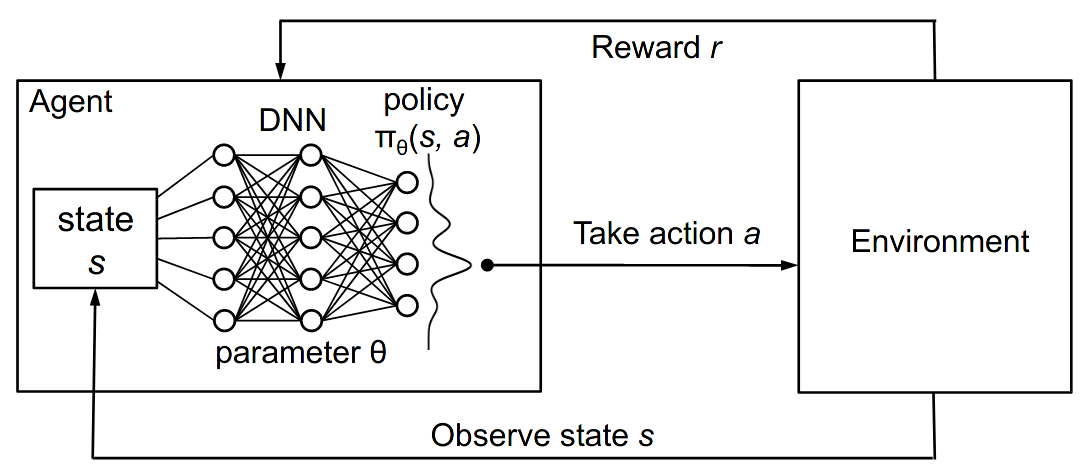
\includegraphics[scale=0.3]{DQN.png}\\
\end{figure}

\subsection{Actions Allowed}
The actions in this scenario, that is the DQN model, is the ordering of the operations we choose to execute. That is, we have $4 = 24$ possible actions on any given input. These are constructed using all possible permutations of $\{0,1,2,3\}$. We then transform this information into 1 hot encoding for ease of use.
\par Consider the set of permutations of $\{0,1,2,3\}$, we can order them lexicgraphically.\\
Given a permutation $\mathbb{P}$, it will have a rank $r$ in the ordering.\\
To convert the permutation into a $1$hot encoding, start with a $24$ element vector $v$ with all $0$s.Then update 
$$v[r]=1$$

\subsection{State Space}
We want the information extracted, i.e. the column wise entropy and the size of the relations, to represent the current state of the environment. Hence, any state is going to be represented as a vector of length $10$, the first $8$ are the column wise entropy and the $9^{th},10^{th}$ are the sizes of the two relations.\\
Note the makes the image of the state space to be a subset of $\mathbb{R}^{10}$. But as entropy is never going to be $0$ and so won't the size of the relations, we can trim it down to $(0,\infty)^{10}$ which is a continuous space.
\par Discretization is a process that divides numeric features into categorical  ones  using  intervals.   Depending  on  the  application and predictive model being used, discretization can bring several benefits, including faster computation time as discrete variables are usually easier to handle compared to numeric ones; and decreases the chances of overfitting since the feature space becomes less complex\cite{DNN_for_stream} . Targeting feature discretization from data streams, a significant milestone was the Partition Incremental Discretization algorithm (PiD)\cite{Pinto2005PartitionID}. While we have not used PiD, it is a powerful tool. PiD discretizes numeric features in two  layers.   The  first  layer  is  responsible  for  computing  a high number of intervals given the arriving data, while the second uses the statistics calculated in the first layer to compute equal frequency partitions.

\subsection{Reward System}
The reward system being used currently is simply taking the number of operations and time required(in micro seconds) as the reward. A more complex state will be when the rewards are not readily available, then another method can be applied as shown in \cite{know_unknown_rewards},\cite{DRL_rewards_problem}.\\
In traditional Q-learning, there is a discount factor involved to discount the moves done later on in the sequence of the game and there is a utility function involved to calculate the utility of each move for each state. The goal of the system is to maximize the expected utility.\\
As the game is a single move game, there is no discounting factor involved neither is a utility function required. We can use the negative of time required or the number of moves required to maximize or minimize with te current positive values. We chose to minimize the positive values.

\subsection{Transition function}
The transition function is the DQN, i.e. the reward determining system, along with the move choosing method. \\
The DQN will output a list of reward, which corresponds to the $24$ moves. Then to choose the optimal action based on reward, we simply scan a chunk of $24$ continuous rewards and associate them to moves.\\
As the game is a single state game, the model of DQN becomes rather simple, and makes it not necessary to choose a discount factor nor do we need to include it into the transition model.\\ 
The method to choose the optimal move is described in the next chapter formally.

\subsection{Assumptions}
Note the amount of information, features extracted from the querying do not fully represent the data set our Neural network can't perform very well. To tackle this, we look at whether the shift in the predicted rewards is similar cross all the moves.\\
Then given data points $(x_{i},y_{i}),(x_{j},y_{j})$ and the DQN $Q_{\theta}$ the condition to check becomes:-
$$y_{i}\leq y_{j}\Rightarrow Q_{\theta}(x_{i})\leq Q_{\theta}(x_{j})$$
If this condition holds, then the predicted optimal move is the actual optimal move. \\
As optimal move implies
$$y_{\text{optimal}}\leq y_{i} \forall i \in [24]$$
This with the previous condition will imply
$$Q_{\theta}(x_{\text{optimal}})\leq Q_{\theta}(x_{i})\forall i \in [24]$$ 
We train a Deep neural network with $70\%$, use the rest of the $30\%$ data for testing and record the results.


\section{Conclusion}
In this chapter we saw :- 
\begin{itemize}
    \item The method use to generate data for the linear road benchmark test cases.
    \item The method implemented to take input, converted $SQL$ queries to $C++$ and extracted features during execution and stored them
    \item Showcased how the extracted features can help with deep reinforcement learning
    \item Showcased the method used to evaluate the performance of DQN. 
\end{itemize}
In the next chapter, we
\begin{itemize}
    \item Formalize the assumptions we made in our evaulation.
    \item Present the categorize/ classification of the data set. Divided into training and testing data.
    \item Visualize the confusion matrix.
    \item Give the true positive, true negative, false positive false negative as well the analysis of the confusion matrix for all $24$ orderings.
    \item Lastly we compare how our predictions fared against the optimal and worst orderings. 
\end{itemize} present the results of our experiments, visualize them
 The method to compute the results are given in the next chapter.
